\section{Testing different Strategies}

\subsection{CPPI Scheme}

Firstly, we will start defining the \textit{benchmark} model. The constant portfolio strategy follows the logic derived from constant relative risk exposure.

This methodology consists in investing a constant proportion $\pi$ of the savings in risky assets (subject to volatility), whilst investing the rest $1 - \pi$ in risk-free assets. The point of this strategy is to present an intuitive straightforward way to control the risk exposure in savings strategies. The simplicity of this approach let us tweak $\pi$ in order to make the investment best suited for the risk aversion profile of each investor individually.

\subsection*{Simulation}

In order to simulate the performance of this kind of strategy, we start assuming that the risky assets follow a simplified geometric brownian motion, with \emph{trend} $\alpha$ and \emph{volatility} $\sigma$. Thus, if the saver invests $x$ in this asset at day $t$, the wealth of the saver at the next day would be $x_{t+1} = (1 + N\qty(\alpha, \sigma)) x_t$.

This way, we construct the scenario of an investor, saving a fixed amount of money - which is denoted as $a$ -   throughout $T/2$ years, and that money being allocated $( 1 - \pi) a$ in the risk-free asset, which we will set with return 0; and $\pi a$ allocated in the risky asset, whose expected return is $\alpha$ and volatility is $\sigma$. Thus, if we set $x_t$ as the wealth at any given time $t$, we can see that

\begin{align}
	x_{t+1} = (1+N(\alpha, \sigma))x_{t}\pi + (1 - \pi)x_{t} + a \textit{.}
\end{align}

At some point in time, our investor will stop saving money and will start consuming it (as in most pension plans), so we just convert that fixed amount of money $a$ to \emph{consumed} money instead of saved. Thus, the evolution of wealth turns out to be:

\begin{align}
	x_{t+1} = x_{t}(1+N(\alpha, \sigma))\pi + (1 - \pi)x_{t} - a \textit{.}
\end{align}

At the end of all $T$ years, the final wealth $X_T$ remaining to the saver is stored. By reproducing this same scheme, we manage to compute tens of thousands of different performances and make some statistics out of them.

\begin{figure}[H]
    \centering
    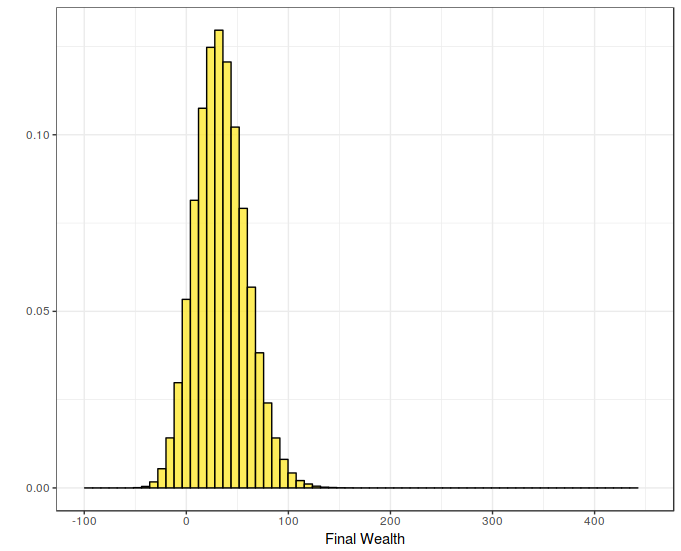
\includegraphics[scale=0.65]{./images/fw_cppi.png}
    \caption{Results of the simulation for the CPPI model. Final wealth obtained for every simulation, where $T=30$, $\mu = 0.0343$, $\sigma = 0.1544$, $a=10$, $\pi = 0.1$}
    \label{fig:cppi_fw}
\end{figure}

If we iterate this process over $10000$ simulations, setting $\pi = 0.1$, $T = 60$, $\alpha = 0.0343$, $\sigma = 0.1544$ and $a = 10$ we get results as shown in figure \ref{fig:cppi_fw}. The first impression we get when looking at the histogram, is that it has the shape of a \textit{Bell Curve}, thus following a \textit{Normal Distribution}, but a simple \textit{Kolmogorov-Smirnov test} would tells us that this is far from being true.


In the following snippet the code necessary to replicate these results in R is shown:
\begin{lstlisting}[language = R]
nsim <- 10000

pi <- 0.1
alpha <- 0.0343 # Expected return of the risky market
sigma <- 0.1544 # Expected volatility of the risky market
a <- 10 # Factor 'a'
years <- 60 # Total time

C <- append(rep(a, round(years/2)),rep(-a, round(years/2)))

X_T <- c()

for (j in 1:nsim){
	x <- c()
	x[1] <- a # Initial wealth

	for (i in 1:(years-1)){
		random <- rnorm(1, mean = alpha, sd = sigma)
		x[i+1] <- x[i]*(1+random)*pi + (1-pi)*x[i] + C[i+1]
	}
	X_T[j] <- x[years]

}
\end{lstlisting}